\include{template}
\cfoot{} %% if no page number is needed

\begin{document}

\begin{header}
FICHE TECHNIQUE

Dilution
\end{header}

Quand on ajoute du solvant à une solution, on réalise une dilution.
La solution obtenue appelée solution fille est moins concentrée que la solution initiale appelée solution mère.

\vspace{20pt}
\begin{Large}
\begin{equation}
\color{bleu_f}
C_\mathrm{m, mère} \times V_\mathrm{mère} = C_\mathrm{m, fille} \times V_\mathrm{fille}
\nonumber
\end{equation}
\end{Large}
\vspace{30pt}

\begin{bframe}
\textbf{Préparation d'une solution par dilution}
\begin{enumerate}
\item Déterminer le volume de solution mère à prélever pour réaliser la solution fille.

\item Préparer la solution.
\end{enumerate}

\begin{multicols}{2}
\paragraph*{Matériel}
\begin{itemize}
\item[•] pipette jaugée ;
\item[•] propipette ;
\item[•] fiole jaugée ;
\item[•] bouchon.
\end{itemize}

\newpage

\paragraph*{Manipulation}
\begin{itemize}
\item[•] Prélever le volume $V_\mathrm{mère}$ de solution mère avec la pipette jaugée.
\item[•] Verser le volume $V_\mathrm{mère}$ de solution mère dans la fiole jaugée.
\item[•] Remplir la fiole jaugée aux trois-quarts, boucher et agiter.
\item[•] Compléter jusqu'au trait de jauge, boucher et homogénéiser.
\end{itemize}
\end{multicols}

\begin{center}
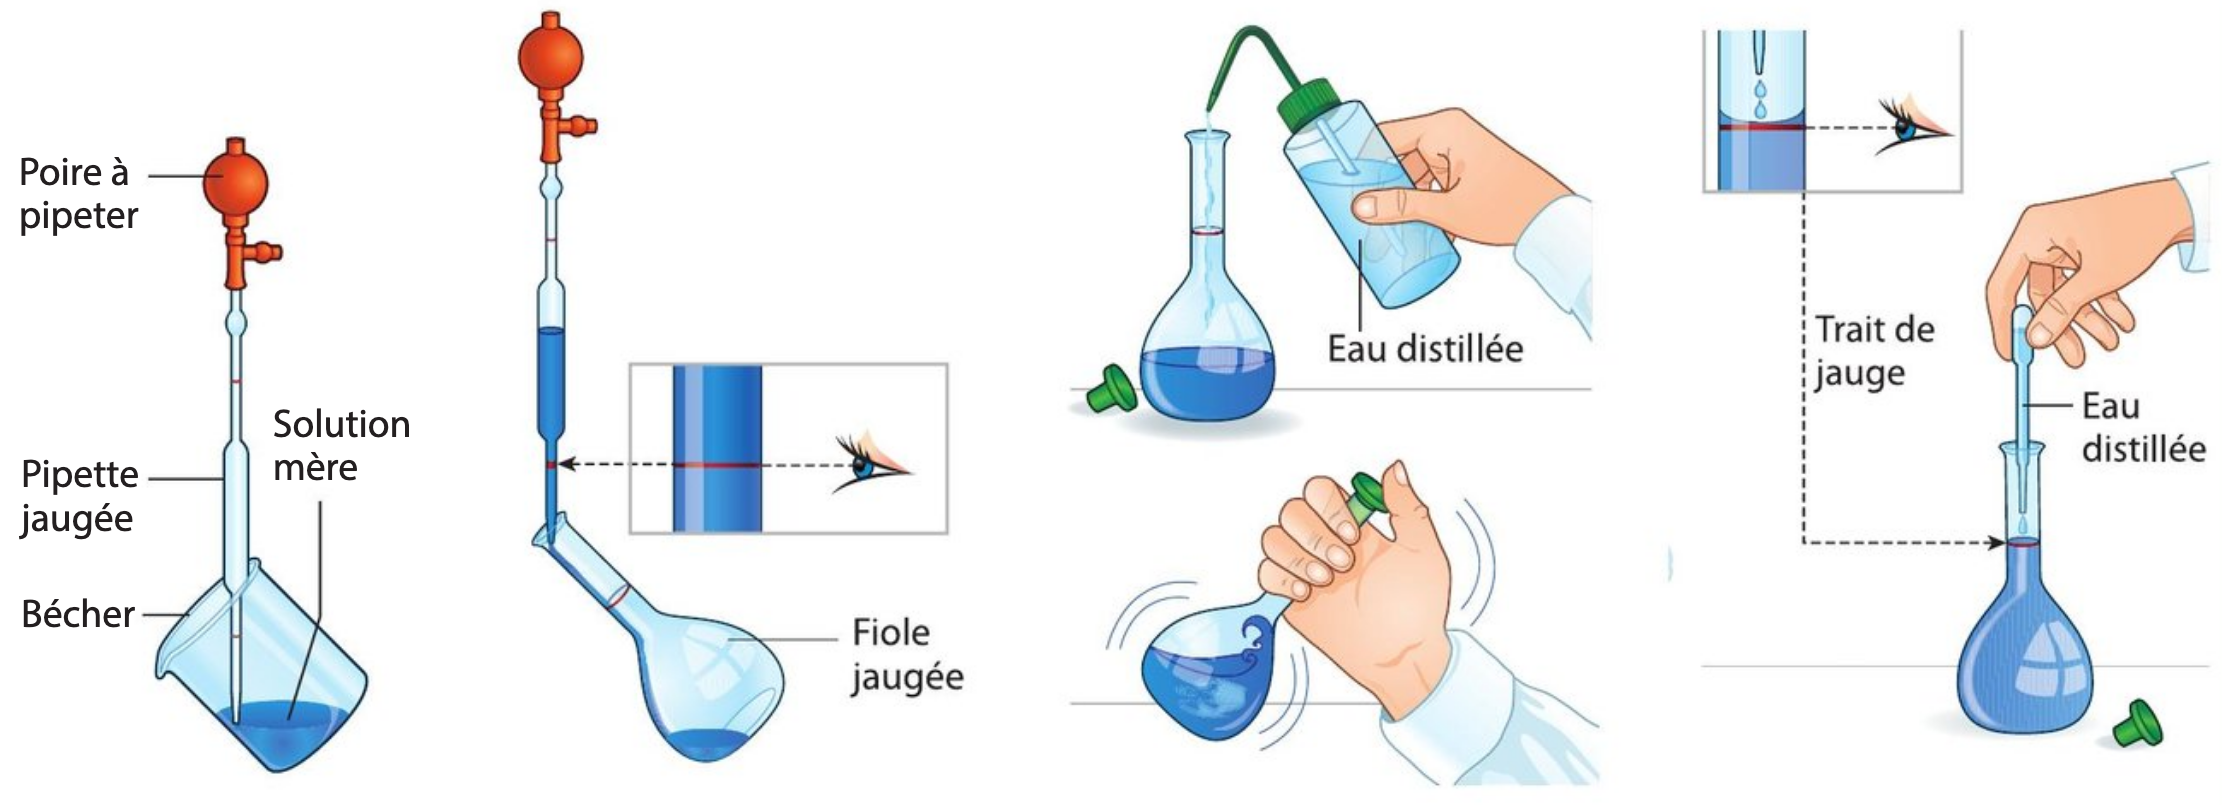
\includegraphics[scale=0.4]{images/dilution.png}
\end{center}

\end{bframe}

\end{document}